\chapter{Análisis de Interfaz de Usuario}
\label{ch:analisis_interfaz_usuario}

La única interfaz de usuario del sistema serán las actividades y diálogos presentes en la aplicación móvil, así pues todas las pantallas identificadas han sido concebidas para un funcionamiento y navegación móvil.

\section{Pantalla de inicio de sesión}

La pantalla de inicio de sesión será la pantalla de entrada a la aplicación para todos los usuarios sin sesión iniciada. Su diseño es el ilustrado en \fref{fig:ui:launch}. Puesto que de primeras sólo se permitirá el inicio de sesión con Google, únicamente se dispondrá un botón para el inicio de sesión que abrirá el selector de cuentas de Google. El inicio sesión puede dirigir al usuario a \nameref{sec:pantalla_creacion_perfil} si es un usuario nuevo o a \nameref{sec:pantalla_principal} para usuarios con perfil ya existente.

\begin{figure}[H]
    \centering
    \begin{minipage}{0.45\textwidth}
        \centering
        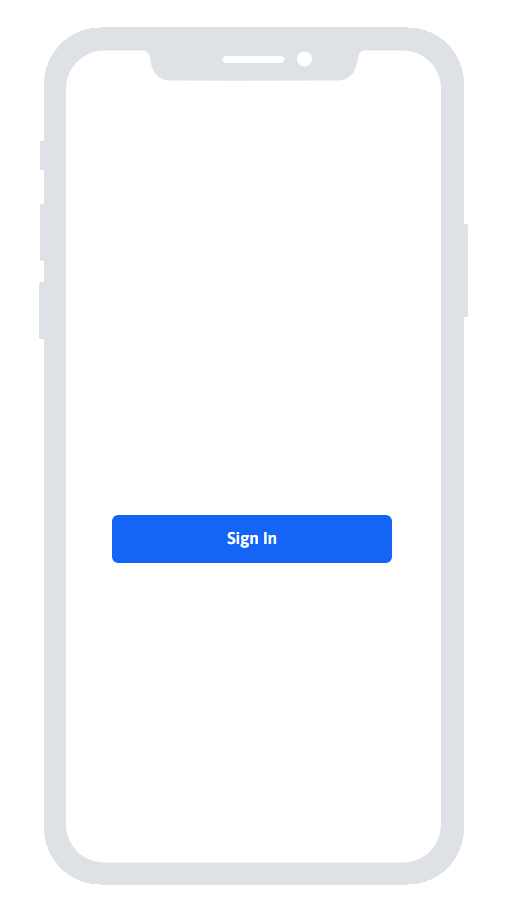
\includegraphics[width=0.9\textwidth]{Analisis/Analisis-Launch.png}
        \caption{Diseño inicial de LaunchActivity}
        \label{fig:ui:launch}
    \end{minipage}\hfill
    \begin{minipage}{0.45\textwidth}
        \centering
        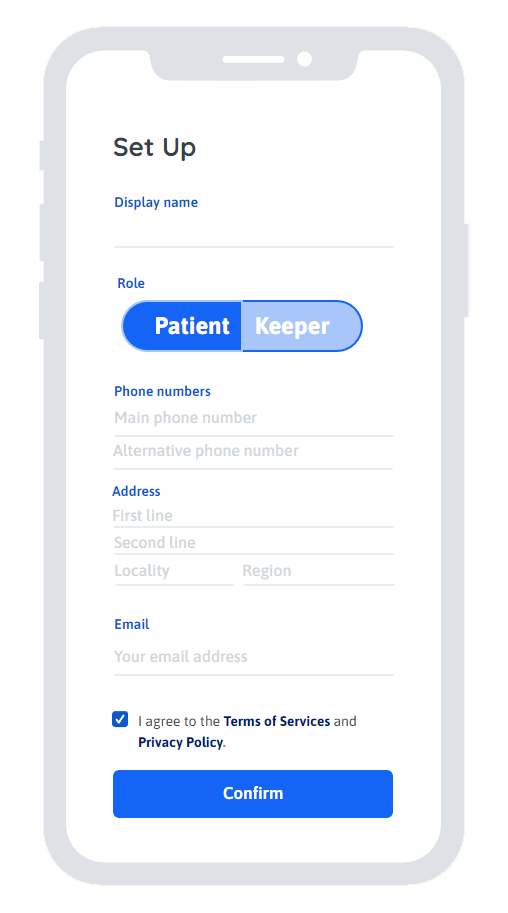
\includegraphics[width=0.9\textwidth]{Analisis/Analisis-SetUp.png}
        \caption{Diseño inicial de SetUpActivity}
        \label{fig:ui:set_up}
    \end{minipage}
\end{figure}

\section{Pantalla de creación de perfil}
\label{sec:pantalla_creacion_perfil}

En esta pantalla se completará el perfil de un usuario recién registrado, en ella se deben disponer campos de texto para que el usuario pueda introducir su nombre visible (\labelcref{req:nombre_usuario}) y su información adicional (\labelcref{req:info_adicional}), además de un selector que le permita elegir entre uno de los dos roles posibles (\labelcref{req:rol_usuario}). Por último, existirá un botón para confirmar los datos introducidos y completar la creación del perfil, lo cuál redirigirá al usuario hacia \nameref{sec:pantalla_principal}. El diseño previo de esta pantalla es el mostrado en \fref{fig:ui:set_up}.

\section{Pantalla principal}
\label{sec:pantalla_principal}

La pantalla principal es el punto de navegación básico de toda la aplicación para los usuarios autenticados. A través de esta pantalla se puede acceder a \nameref{sec:pantalla_vinculos}, \nameref{sec:pantalla_feed}, \nameref{sec:pantalla_geolocalizacion}, \nameref{sec:pantalla_tareas} y \nameref{sec:pantalla_notificaciones}. Su diseño es \fref{fig:ui:main}.

\begin{figure}[H]
    \centering
    \begin{minipage}{0.45\textwidth}
        \centering
        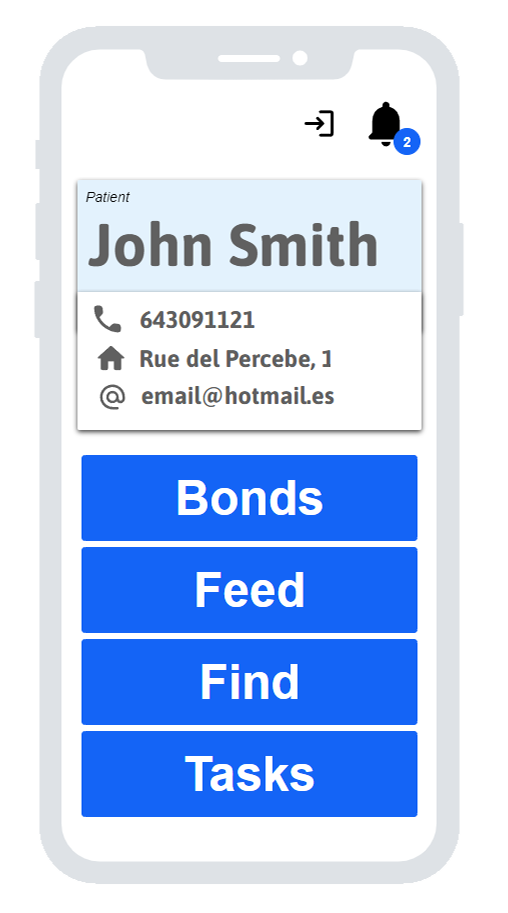
\includegraphics[width=0.9\textwidth]{Analisis/Analisis-Main.png}
        \caption{Diseño inicial de MainActivity}
        \label{fig:ui:main}
    \end{minipage}\hfill
    \begin{minipage}{0.45\textwidth}
        \centering
        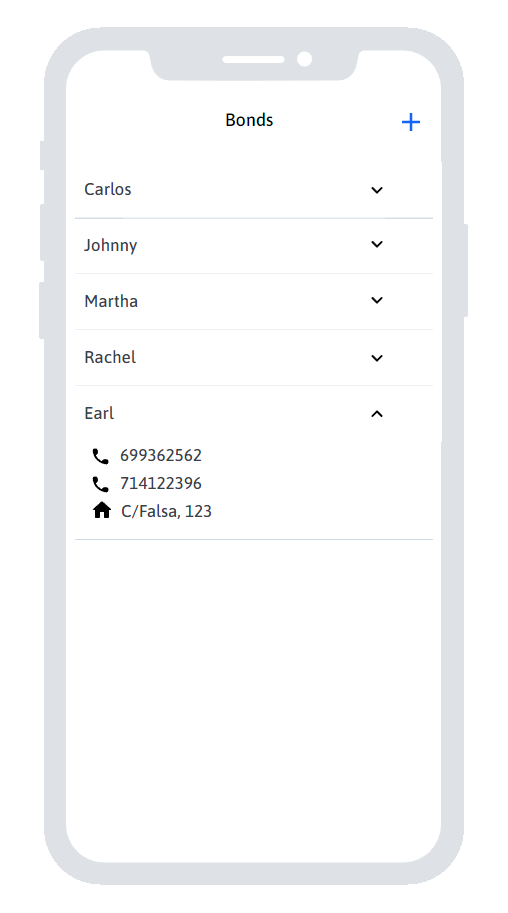
\includegraphics[width=0.9\textwidth]{Analisis/Analisis-Bonds.png}
        \caption{Diseño inicial de BondsActivity}
        \label{fig:ui:bonds}
    \end{minipage}
\end{figure}

\section{Pantalla de vínculos}
\label{sec:pantalla_vinculos}

En la pantalla de vínculos se listan los usuarios asociados. Cada uno de estos usuarios listados podrá ser desplegado para consultar su información de contacto. Además de esta información también habrá un botón para crear un nuevo vínculo, que en el caso de los Pacientes mostrará un código QR de vinculación y en el de los Cuidadores abrirá la cámara para escanearlo. La \fref{fig:ui:bonds} muestra su primer diseño.

\begin{figure}[H]
    \centering
    \begin{minipage}{0.45\textwidth}
        \centering
        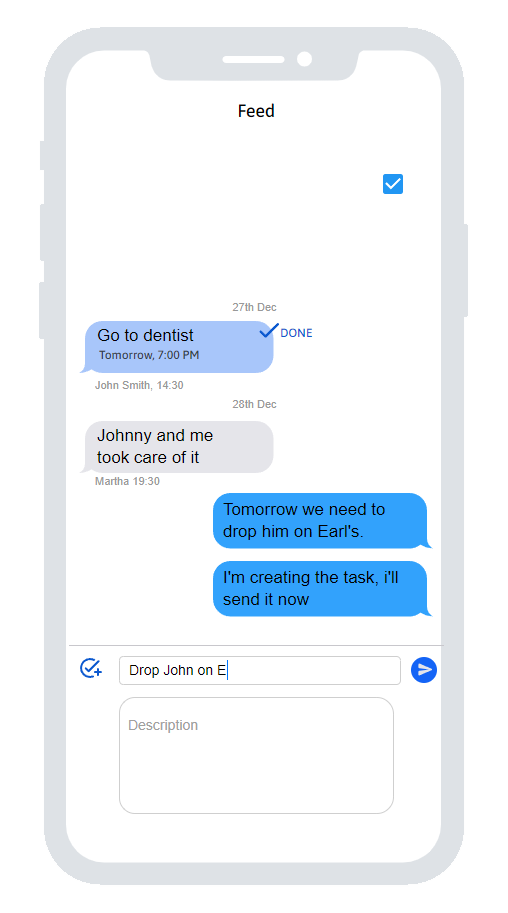
\includegraphics[width=0.9\textwidth]{Analisis/Analisis-Feed.png}
        \caption{Diseño inicial de FeedActivity}
        \label{fig:ui:feed}
    \end{minipage}\hfill
    \begin{minipage}{0.45\textwidth}
        \centering
        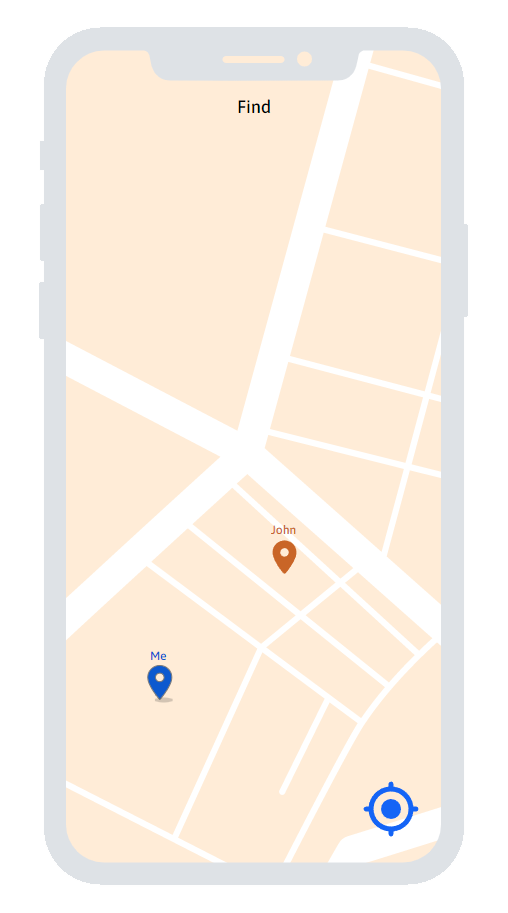
\includegraphics[width=0.9\textwidth]{Analisis/Analisis-Find.png}
        \caption{Diseño inicial de LocationActivity}
        \label{fig:ui:location}
    \end{minipage}
\end{figure}

\section{Pantalla del feed}
\label{sec:pantalla_feed}

La pantalla que contiene el chat entre usuarios asociados. Contendrá las funciones habituales de un chat como la lista de mensajes, diferenciando los enviados y los recibidos; fechas y horas de envío de mensajes; o un campo de texto y un botón para enviar los mensajes. Aparte de eso también dispondrá de un botón para cambiar de modo al de creación de tareas, desplegando un área de texto para la descripción. Dichas tareas también tendrán un aspecto diferenciado de los mensajes y mostrarán visualmente su estado con una caja de verificación que también podrá ser pulsada para modificarlo. Este chat puede verse en la \fref{fig:ui:feed}.

\section{Pantalla de geolocalización}
\label{sec:pantalla_geolocalizacion}

El servicio de geolocalización de los usuarios se servirá por medio de una actividad compuesta de un mapa decorado con los marcadores de la ubicación de los distintos usuarios que se encuentren compartiendo su ubicación en esos momentos y que se irá actualizando a medida que dichos usuarios se desplacen. Aparte de esto también habrá un botón para centrar el mapa sobre la posición del usuario y permitir que siempre pueda recuperar la referencia. Una muestra de todo eso se ofrece en \fref{fig:ui:location}.

\begin{figure}[H]
    \centering
    \begin{minipage}{0.45\textwidth}
        \centering
        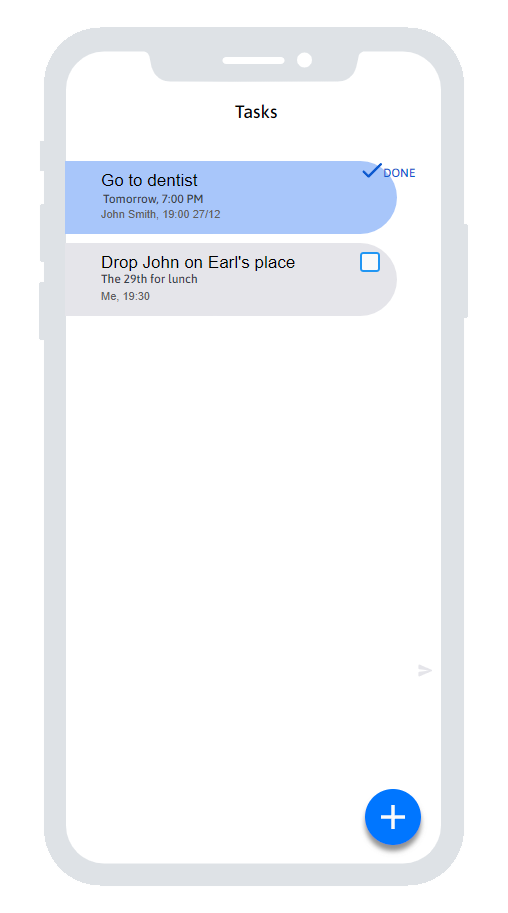
\includegraphics[width=0.9\textwidth]{Analisis/Analisis-Tasks.png}
        \caption{Diseño inicial de TasksActivity}
        \label{fig:ui:tasks}
    \end{minipage}\hfill
    \begin{minipage}{0.45\textwidth}
        \centering
        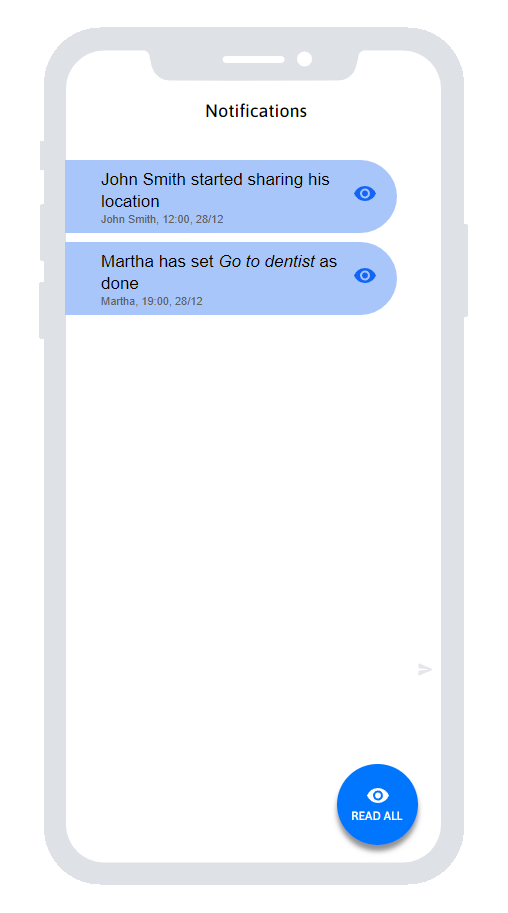
\includegraphics[width=0.9\textwidth]{Analisis/Analisis-Notifications.png}
        \caption{Diseño inicial de NotificationDialog}
        \label{fig:ui:notification}
    \end{minipage}
\end{figure}

\section{Pantalla de gestión de tareas}
\label{sec:pantalla_tareas}

La última actividad ofrecerá un listado de las tareas relevantes del usuario con toda la información importante (\labelcref{req:info_tarea}) de las mismas, así como una representación visual del estado de estas, estado que podrá modificarse con una caja de verificación. Aparte de esto, contará también con un botón para crear notificaciones que desplegará un creador de tareas similar al presente en el diseño de \nameref{fig:ui:feed}. La vista preliminar de esta actividad es la \fref{fig:ui:tasks}.

\section{Pantalla de notificaciones}
\label{sec:pantalla_notificaciones}

Este pantalla no será una actividad sino un diálogo sobre la \nameref{fig:ui:main} que será desplegado al utilizar el botón con el icono de la campana. Esta actividad listará todas las notificaciones no leídas por el usuario y cada una de ellas contará con un botón para marcarla como leída. Algo que también podrá hacerse con el botón de marcar todas como leídas, \fref{fig:ui:notification}.

\section{Mapa de navegación}

El mapa de navegación de las pantallas anteriores es el ilustrado en \fref{fig:ui:navegacion}. Aquellas pantallas con fondo azul son pantalla privadas que requieren autenticación para acceder.

\begin{figure}[H]
    \centering
    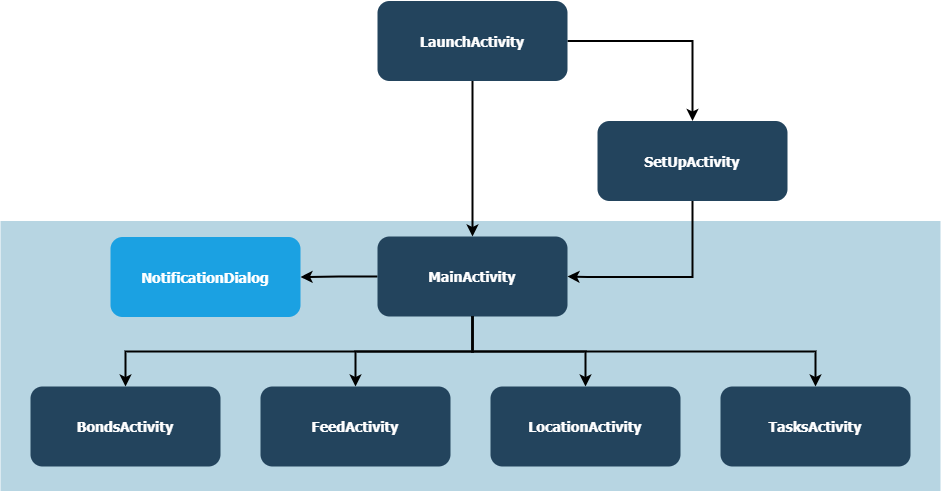
\includegraphics[width=0.9\textwidth]{Analisis/MapaNavegacionAnalisis.drawio.png}
    \caption{Propuesta de mapa de navegación}
    \label{fig:ui:navegacion}
\end{figure}